\chapter{Conception}
In order to conceptualize the bandwidth limiter for \acs{SCIONLab} properly, we first need to formalize the requirements. We want to achieve the following:

\begin{enumerate}
\item[$\bullet$]The \acs{SCIONLab} administrators should be able to set a maximal bandwidth that is available to the user-\acsp{AS}.
\item[$\bullet$]The users should be able to set an upper limit for the bandwidth in the range of $[0,x]$ where $x$ is the bandwidth limit set by the \acs{SCIONLab} administrators.
\item[$\bullet$] The above-mentioned limits should be enforced automatically by only making configurations on the \acsp{AP}.
\end{enumerate}

We split up these three requirements into two sections. The first two belong to the front end of the project, where as the third requirement is part of the back end.

\section{Front End}

The front end part of the project is all about the \acs{SCIONLab} server. The implementation of that server can be found on \href{https://github.com/ManuelMeinen/scionlab/tree/bw-limit}{github.com}\cite{meinen2019scionlab}. There is already a configuration page, where the users can set the desired configuration for their user-\acsp{AS}. On the same configuration page we simply add a field, where the users can insert a bandwidth limit between 0 and the limit set by the \acs{SCIONLab} administrators. Other bandwidth limits get already rejected by the form.
\\
The \acs{SCIONLab} server stores information about the entire topology of the \acs{SCIONLab} network, including information about the links from the \acsp{AP} to the user-\acsp{AS}. Per link there is a field that stores the maximal bandwidth for that link. This field already exists but is currently not used. Therefore we simply set that attribute to the bandwidth limit that the user chose.
\\
The \acs{SCIONLab} server regularly generates files according to its data model that are then sent to the \acsp{AP}, in order to configure them for newly added or updated user-\acsp{AS}. These files are packed in a tarball and then delivered and unpacked on the \acsp{AP}. We can use this mechanism to deliver the information we need to the \acsp{AP}, in order to enforce the bandwidth limitations. So we simply add a \ac{JSON}-file called \textit{link\_info.json} to that tarball, which holds the information we need to perform bandwidth limitations.

\section{Back End}

The back end part is all about configuring the \acsp{AP} in a way that the bandwidth limits that are specified in the \textit{link\_info.json} file are put into effect. We do that using the \acs{TC} utility. However, there is no \acs{API} to use \acs{TC} in an automated way. Therefore we need to write a wrapper program that configures \acs{TC} via the command line. This wrapper program is written in Python and is available on \href{https://github.com/ManuelMeinen/SCIONLab_Bandwidth_Limiter}{github.com}\cite{meinen2019scionlabBwLimiter}. Further details on how this program is implemented can be found in chapter \ref{Implementation}.
\\
Furthermore, we have to make some design decisions. Especially, we have to decide on how to build up the \acs{TC} logic. Figure \ref{QDISC-Set-up} shows in an abstract way how \acsp{QDISC}, classes and filters are set up on both physical as well as virtual interfaces and how they are related.
\\
Ingress, as well as egress traffic, firstly goes through the physical interface. Ingress traffic is then redirected by the \textit{ingress} \acs{QDISC} (with handle ffff) to a virtual interface. On the virtual interface, ingress traffic is handled the same way as egress traffic is on the physical interface. In both cases we use an \acs{HTB}-\acs{QDISC}. To make these \acsp{QDISC} more distinguishable, we define the handle for a \acs{QDISC} on a physical interface to be 1 and 2 if it is on a virtual interface. In both cases we define one class for each connection to a user-\acs{AS} and set the corresponding bandwidth limit to its leaf-\acs{QDISC}. Furthermore we define a default class, which limits all traffic going through this interface that doesn't match with any filter to the default bandwidth. Each class has the \acs{AS}-id as a class id, which is unique to each \acs{AS}. The default classes have a class id of 9999. Each \acs{HTB}-\acs{QDISC} has as many classifier filters as there are user-\acsp{AS} plus one implicit one for the default class (represented as arrows in figure \ref{QDISC-Set-up}). The \textit{ingress} \acs{QDISC} has only one filter, which is a redirect filter that redirects ingress traffic of the physical interface to the virtual interface.
\begin{figure}[h]
	\centering
	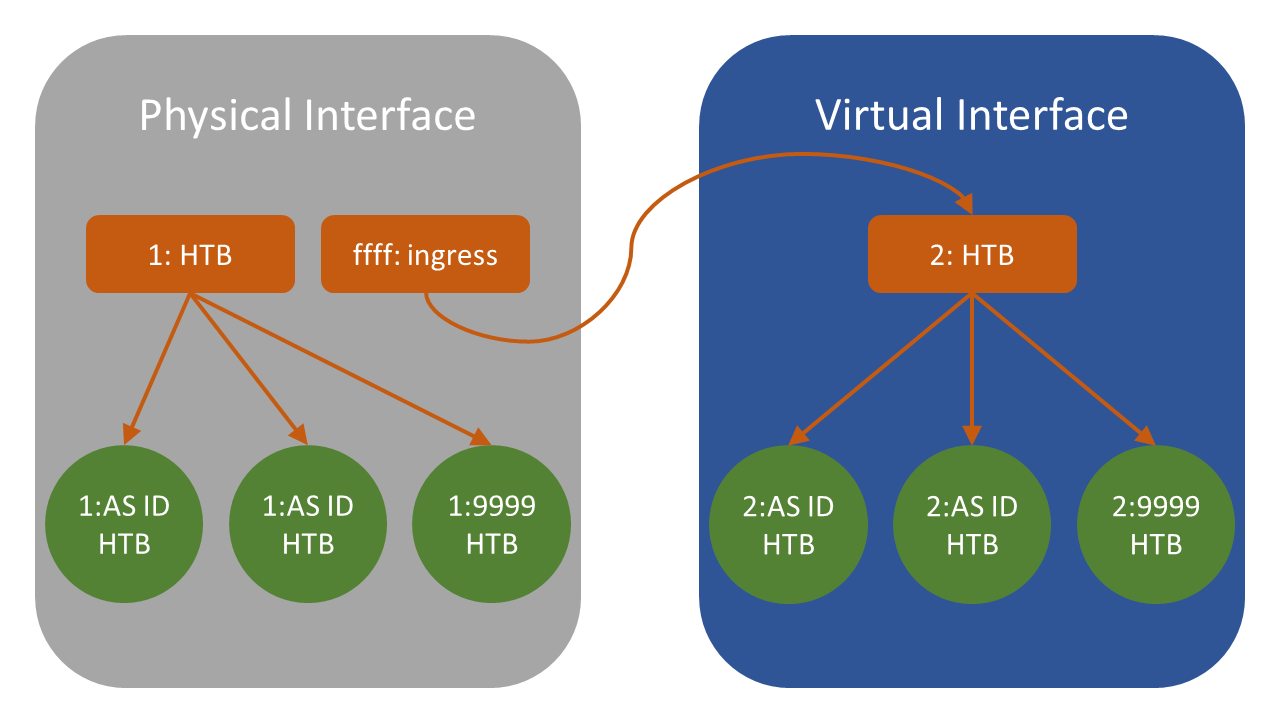
\includegraphics[width=\textwidth]{img/QDISC-Set-up.png}
	\caption{QDISC/Class Hierarchy}
	\label{QDISC-Set-up}
\end{figure}